METHODS AND RESULTS FOR REMOVING INFORMATION FROM THE ALREADY PUBLISHED PAPER

\subsubsection{Influences on receiving thrombolysis across a patient cohort}

Model accuracy was measured using stratified 5-fold cross validation. Overall accuracy was 85.0\% (83.9\% sensitivity and specificity could be achieved simultaneously). The model predicted hospital thrombolysis use at each hospital with very good accuracy (r-squared = 0.977, with a mean absolute error of 1.1 percentage points).

Figure 2 shows the relationship between patient level feature values and their odds of receiving thrombolysis (shown as their SHAP values). Key observations are:
\begin{enumerate}
    \item The odds of receiving thrombolysis reduced 9-fold over the first 120 minutes of arrival-to-scan time, varied 30-fold with stroke severity, reduced 3-fold with estimated rather than precise stroke onset time, reduced 6-fold with increasing pre-stroke disability, reduced 4-fold with onset during sleep, reduced 5-fold with use of anticoagulants, reduced 2-fold between 80 and 110 years of age, reduced 3-fold between 120 and 240 min of onset-to-arrival time and varied 13-fold between hospitals.
    \item The majority of between-hospital variance was explained by the hospital, rather than by the differences in local patient populations.
\end{enumerate}


\begin{figure}
    \centering
    \begin{subfigure}{0.8\textwidth}
      \centering
      \captionsetup{width=.9\linewidth}
      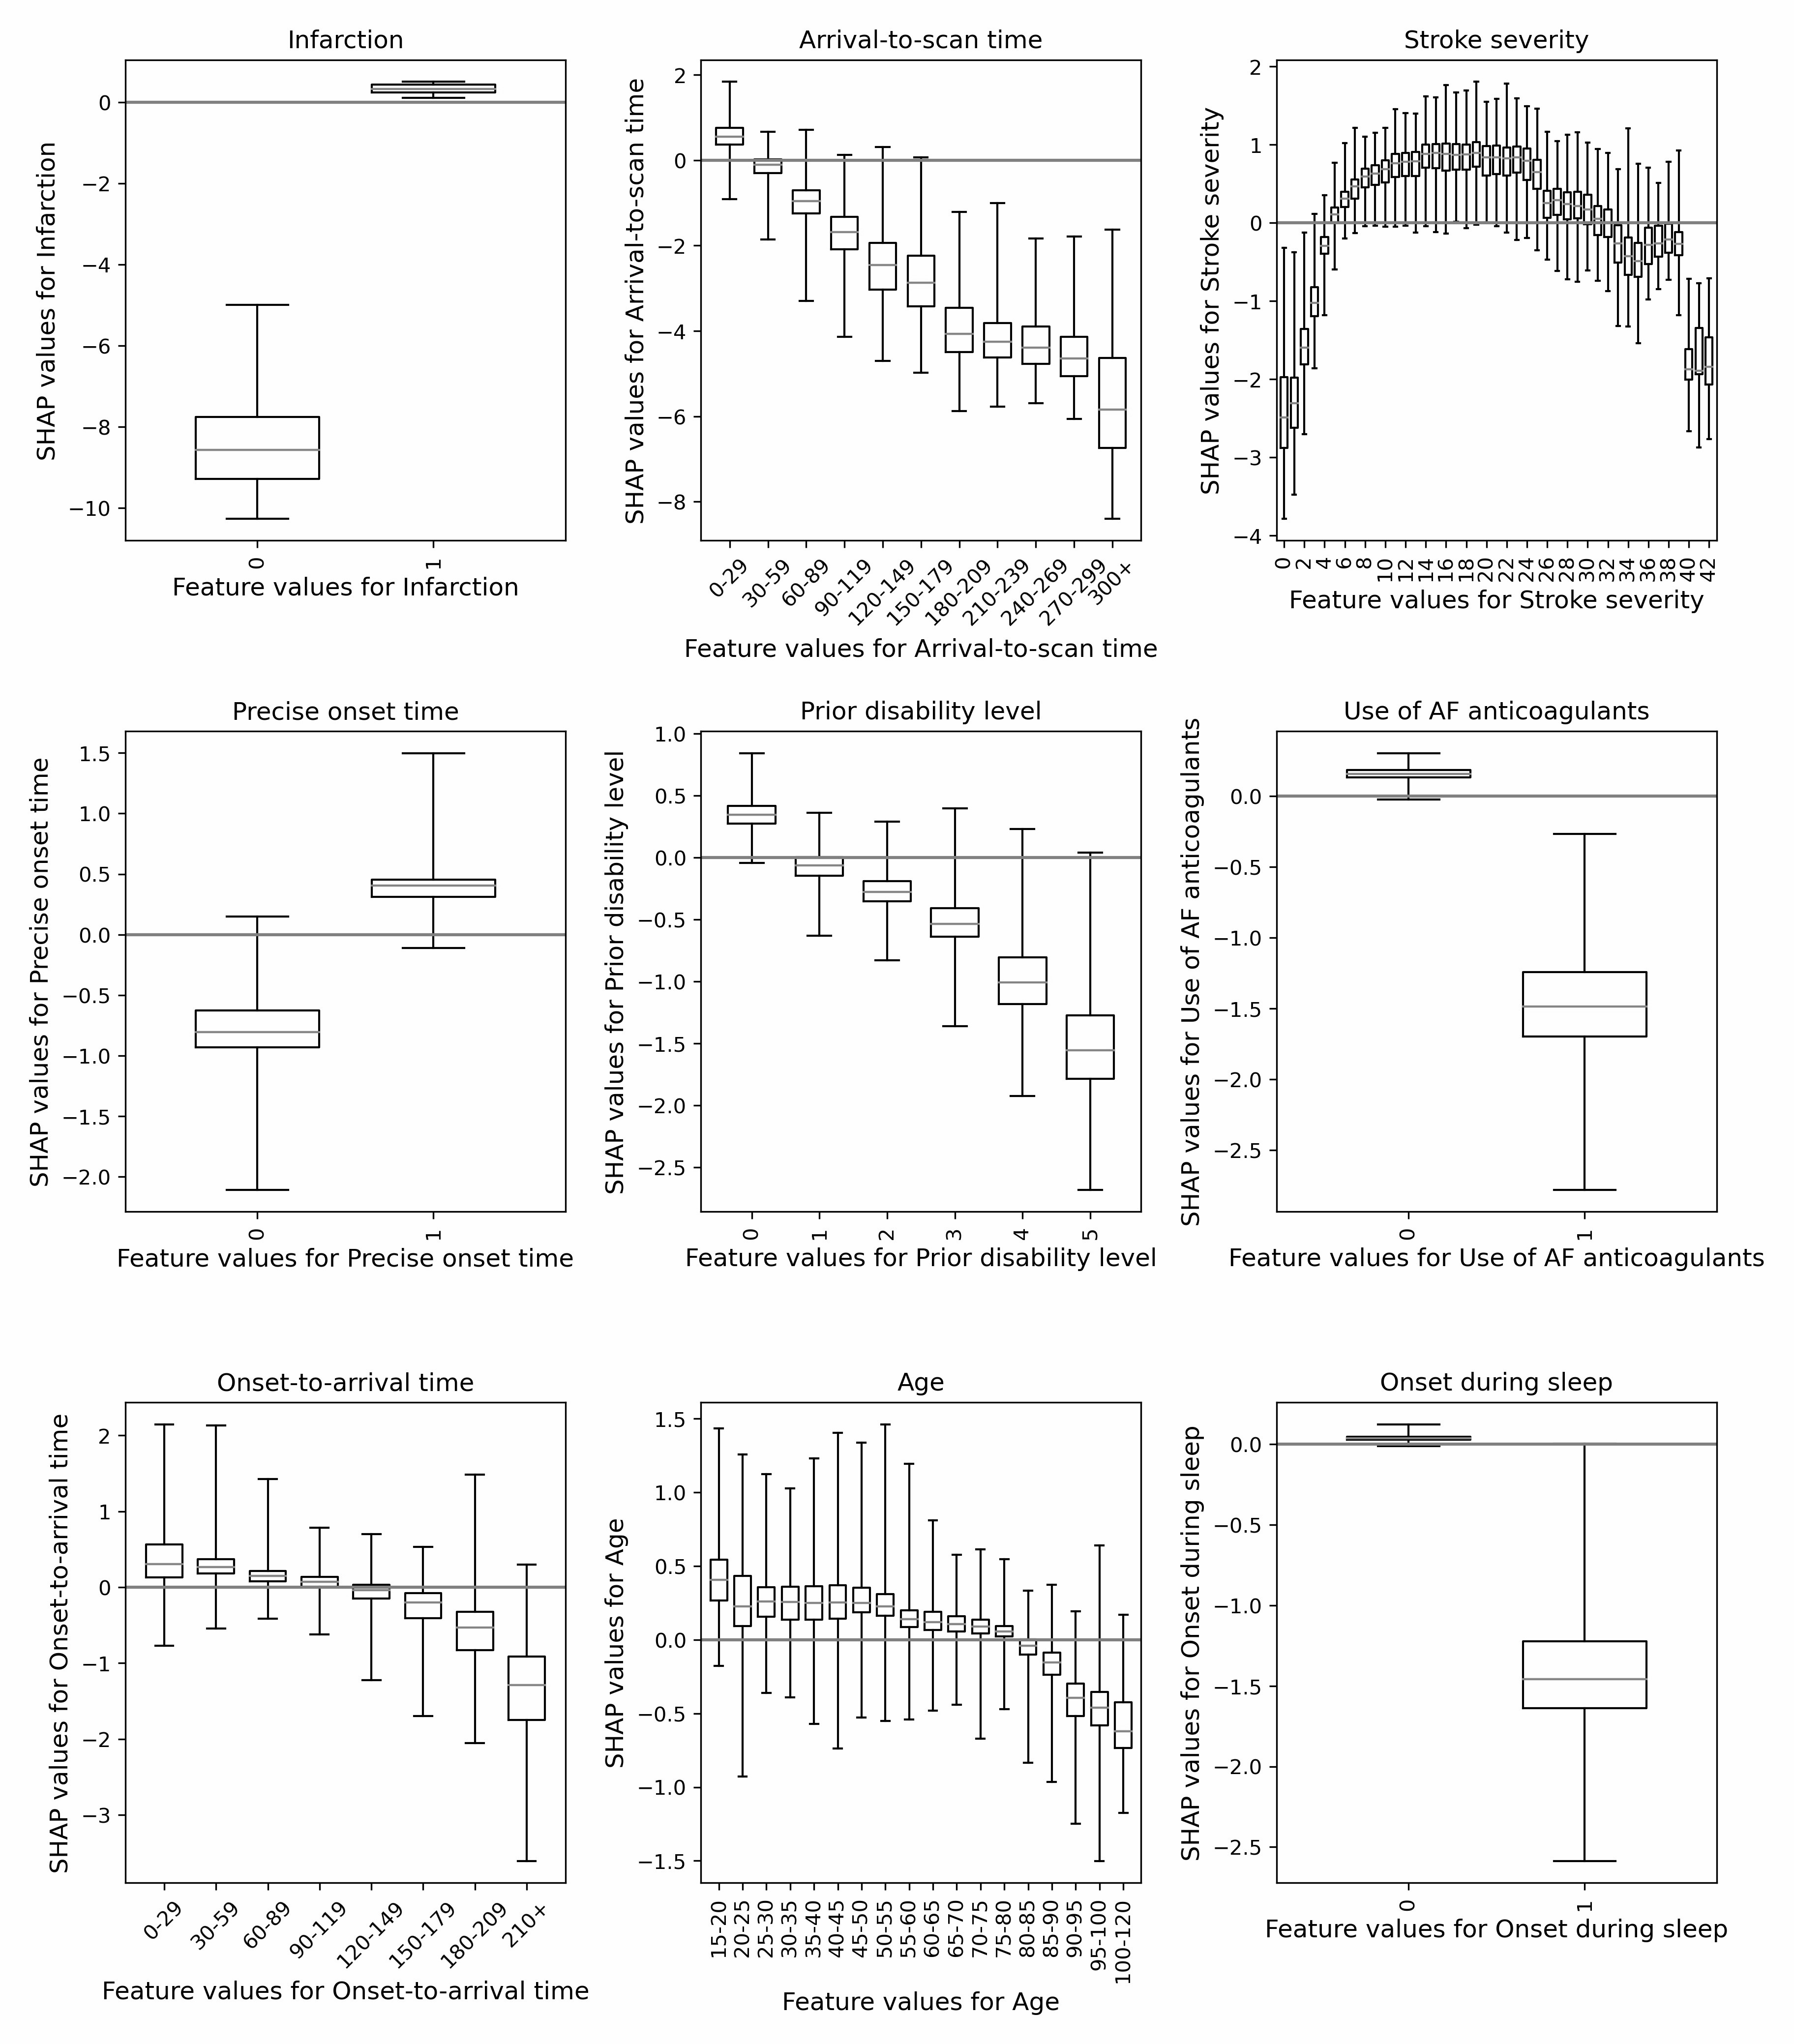
\includegraphics[trim={0 0 0 1.2cm}, clip, width=0.95\linewidth]      {images/p2_patient_shap.jpg}\\
        \caption{Box plots showing the relationship between SHAP values  (log odds of receiving thrombolysis) and feature values. Box plots show inter-quartile range (box), median (mid-line in box), and range (whiskers). The plots are ordered in ranked feature importance (using the mean absolute SHAP value across all instances).}
        \label{fig:global_shap}
    \end{subfigure}
    \hfill
    \begin{subfigure}{0.8\textwidth}
      \centering
      \captionsetup{width=.9\linewidth}
      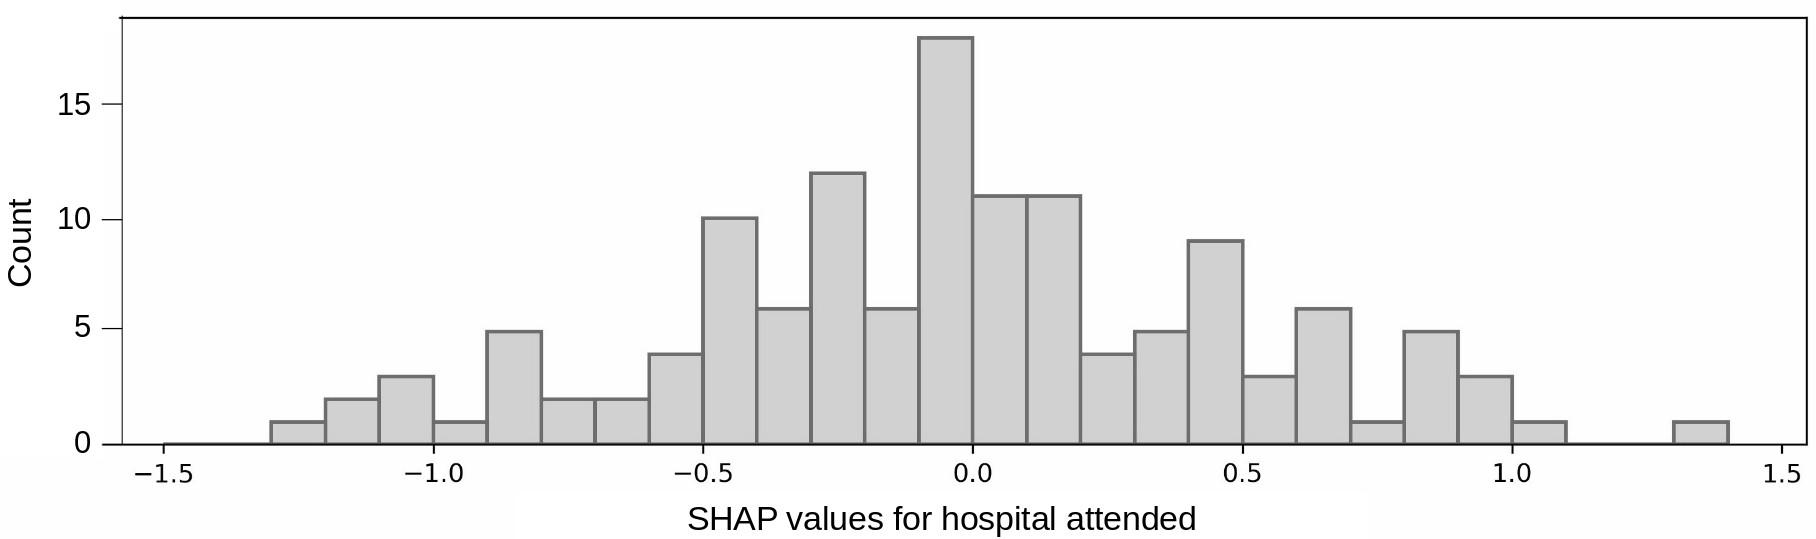
\includegraphics[trim={0 0 0 0.1cm}, clip, width=1\linewidth]    {images/p2_hosp_shap.jpg}
    \caption{Histogram showing the frequency of SHAP values (log odds of receiving thrombolysis) for the hospital attended.}
    \label{fig:hospital_shap}
    \end{subfigure}
  \caption{Plots showing the relationship between SHAP values and feature values for predicting thrombolysis use. Top: Violin plots showing the relationship between SHAP values and feature values. The horizontal line shows the median SHAP value. Bottom: Histogram showing the frequency of the mean SHAP value for the hospital attended.}
    \label{fig:shap_outcome_model1}
\end{figure}

%%%%%%%%%%%%%%%%%%%%%%%%%%%%%%%%%%%%%%%%%%%%%%%%%%%



METHODS


***


(1) XBGoost  \cite{chen_xgboost_2016} (machine learning model) for predicting thrombolysis use, (2) XBGoost (machine learning model) for predicting patient clinical outcome, and (3) discrete event simulation for modelling the acute stroke pathway. 


\subsection{Quantitative research: models}

Three types of models were created: (1) XBGoost  \cite{chen_xgboost_2016} (machine learning model) for predicting thrombolysis use, (2) XBGoost (machine learning model) for predicting patient clinical outcome, and (3) discrete event simulation for modelling the acute stroke pathway. 

\subsubsection{Quantitative research: Data for models}

All of the models used data extracted from the Sentinel Stroke National Audit Programme (SSNAP), the national stroke registry for England, Wales and Northern Ireland. SSNAP contains patients admitted to all acutely-admitting hospitals in England and Wales, with a case ascertainment of over 90\% when compared to administrative data (Hospital Episode Statistics). Data is used for patients with an out-of-hospital stroke onset that arrived at an acute stroke team (with at least 250 stroke admissions, and which delivered thrombolysis to at least 10 patients in the study period) in England and Wales by ambulance after their stroke onset. See individual models for further details of the data used for each model.

\subsubsection{Quantitative research: Feature selection}

Each of the XGBoost models were trained on features that describe the patients characteristics, their acute stroke pathway timings, attended hospital, and, for the outcome model, use/time to thrombolysis. In order to simplify each of the XGBoost models (for enhanced explainability) we selected those features most predictive of the target feature. Features were selected by forward-feature selection, identifying one feature at a time that led to the greatest improvement in accuracy as measured by Receiver Operating Characteristic (ROC) Area Under Curve (AUC). We repeated this process to identify the top 25 features, and used these results, together with feedback from discussions with clinicians, to identify the features to include in our machine learning models. The discrete event simulation model used features to describe the process from stroke onset to disability at inpatient discharge. See table n in the appendix showing the fields used in each model.

\subsubsection{Quantitative research: Accuracy}

Each of the XGBoost models were trained using stratified 5-fold cross-validation to test the accuracy of the model, for feature selection, and to test reproducibility of patterns detected (in 5-fold cross validation the data is split into 5 different 80:20 train/test splits with each patient being in one, and only one, test set). The results from the model fitted on the first k-fold split were used to investigate the relationships between feature values and their contribution to the prediction.

\begin{enumerate}
    \item Machine learning model to predict thrombolysis use: Decision-making (choice of thrombolysis) were modelled with machine learning, learning which patients would likely be given thrombolysis at each stroke team.
    \item Machine learning model to predict patient clinical outcome: to train a model to predict outcome from thrombolysis alone, we excluded any patient who had received thrombectomy. We trained XGBoost models to predict two representations of the mRS score at discharge from the other feature values: 
    \begin{enumerate}
        \item a multiclass classification model that predicts a probability distribution across the seven mRS levels
        \item a set of six independent XGBoost models to predict the likelihood of an ischaemic stroke patient attaining any given mRS threshold at discharge (for each mRS threshold, we refer to being at or lower than that threshold as a \textit{'same or better}' or '\textit{good outcome}'). 
    \end{enumerate}
\end{enumerate}


\subsection{Stroke outcome machine learning model}

The machine learning model predicting disability/death at discharge (mRS) is described in more detail in a companion paper \cite{pearn_are_2024}. Briefly, we used XGBoost \cite{chen_xgboost_2016} to predict outcome (mRS level) based on the following features:

\begin{enumerate}
    \item \textit{Prior disability level}: Disability level (mRS) before stroke
    \item \textit{Stroke severity}: Stroke severity (NIHSS) on arrival
    \item \textit{Stroke team}: Attended hospital
    \item \textit{Age}: Age (as middle of 5 year age bands)
    \item \textit{Onset to thrombolysis time}: Time from onset to receiving thrombolysis (minutes). Set to 9999 if did not receive thrombolysis.
    \item \textit{Any afib diagnosis}: Patient has a diagnosis of atrial fibrillation (either on arrival or new)
    \item \textit{Precise onset known}: Onset time recorded is precise time (not a best estimate)
\end{enumerate}

The model is trained with two different representations of the target feature: 
\begin{enumerate}
    \item a single multiclass XGBoost classification model that predicts a probability distribution across the seven mRS levels
    \item a set of six independent XGBoost models to predict the likelihood of a patient attaining any given mRS threshold at discharge (for each mRS threshold, we refer to being at or lower than that threshold as a \textit{'same or better}' or '\textit{good outcome}'). 
\end{enumerate}

\subsubsection{XGBoost model accuracy}

Model accuracy (using stratified 5-fold cross-validation) is reported as: percent correct, percent correct within one mRS category, sensitivity and specificity, ROC AUC, and confusion matrix. For the thrombolysis use model, the predicted thrombolysis rate was compared with actual thrombolysis use at hospital-level.

\subsubsection{SHapley Additive exPlanation (SHAP) values}

We sought to make our models explainable using SHAP values \cite{lundberg_unified_2017}. SHAP provides a measure of the contribution of each feature value to the final predicted value for the target feature. The SHAP values for each feature are comprised of the feature’s main effect (the effect of that feature in isolation) and all of the pairwise interaction effects with each of the other features. SHAP values provided the influence of each feature as the change in log-odds of having a certain value (SHAP values expressed as log-odds are additive; the final model log-odds prediction for an individual is the sum of all its feature SHAP values and the models baseline SHAP value, which is common across all individual predictions). A positive SHAP value represents that the corresponding feature value increases the likelihood for that individual to have that value, and a negative SHAP value represents that the feature value reduces the likelihood for that patient to have that value. SHAP values can be assessed \textit{locally} at patient level, and \textit{globally} at patient cohort level to understand general patterns of how the target feature differs by each of the patient, pathway, and hospital characteristics. We also illustrated our model with \textit{prototype} patients which vary patient characteristics in a controlled way.

\subsubsection{Counterfactual treatment: Predicting if a patient would be likely to have a better outcome with or without thrombolysis}

We used the first k-fold \textit{thrombolysis outcome} model to calculate the counterfactual outcome for each treatment option (with and without thrombolysis) for the 15,680 patients in the first k-fold test set. We represented patients as receiving thrombolysis by setting the feature \textit{onset to thrombolysis time} to the sum of the recorded pathway durations for the patient (\textit{onset to arrival} and \textit{arrival to scan}) and added on the median \textit{scan to thrombolysis time} of their attended hospital. The median \textit{onset to thrombolysis time} for the 15,680 patients is 162 minutes (range 27 to 316 minutes). We represented patients as not receiving thrombolysis by setting the feature \textit{onset to treatment time} to 9,999 minutes. We translated the resulting two predicted probability distributions of disability at discharge (with and without thrombolysis) into a binary feature to represent whether the patient was predicted to have a better outcome receiving thrombolysis. We used a conservative definition to determine whether a patient has a better outcome with treatment from the two probability distributions, where both of these criteria must be met: 

\begin{enumerate}
    \item A reduction in probability-weighted mRS (a measure of the mid-point location of disability; it is the sum of each mRS outcome multiplied by the probability of that outcome occurring).
    \item A reduction in the likelihood of a very bad outcome (mRS 5-6, complete dependency or death).
\end{enumerate}

\subsubsection{Hospital trade-off between maximising benefit from thrombolysis and minimising risk of harm from thrombolysis}

We used a XGBoost \textit{thrombolysis decision} model to predict the thrombolysis decision of each of the 15,680 patients in the test set at each of the 111 stroke teams (by setting their feature \textit{stroke team} value to each of the stroke teams in turn). We used the \textit{thrombolysis outcome} model to predict the two mRS distributions at discharge (with and without treatment) for each of the 15,680 patients, and translated this into a binary feature to represent whether the patient was predicted to have a better outcome receiving thrombolysis. To remove the affect that hospital attended has on patient outcome at discharge, for each of the 15,680 patients in the first k-fold test set, we predicted outcomes at a hospital with the most neutral contribution to outcomes. To compare maximising benefit from thrombolysis and avoiding potential harm from thrombolysis we defined measures for \textit{sensitivity} and \textit{specificity} of treatment. \textit{Sensitivity} was calculated as the proportion of patients who were predicted to benefit from thrombolysis (from the \textit{thrombolysis outcome} model) who were predicted to receive thrombolysis at each team (from the \textit{thrombolysis decision} model). \textit{Specificity} was calculated as the proportion of patients who were predicted not to benefit from thrombolysis (from the \textit{thrombolysis outcome} model) who were not predicted to receive thrombolysis at each team (from the \textit{thrombolysis decision} model). A low \textit{sensitivity} would indicate a higher likelihood of not treating people who would benefit from thrombolysis, and a low \textit{specificity} would indicate a higher likelihood of treating people who would not benefit from thrombolysis.

\subsubsection{Quantitative research: Model to simulate the acute stroke pathway}

The model to simulate the acute stroke pathway is described in more detail in a companion paper \cite{pearn_are_2024}. Briefly, process flow was modelled by sampling from distributions of historic flow for each stroke team, and machine learning models were used to decide whether the patient received thrombolysis \cite{pearn_are_2024} and to predict the patient clinical outcome (predicting disability/death at discharge) \cite{pearn_are_2024}).

Code, with demonstration, is available at \url{https://github.com/samuel-book/samuel_2_demo}.

%Code, with demonstration, is available \cite{allen_samuel_code_2024}.

\subsubsection{Quantitative research: Acute stroke pathway model, prototype patients}

To help compare decision-making and outcomes across stroke teams we exemplified differences using \textit{prototype patients}. These prototype patients captured a range of features known to affect decisions to treat, and to affect outcomes, and included an \textit{ideal} candidate for thrombolysis. The prototype patients used were:

\begin{enumerate}
    \item \textit{Ideal}: Onset-to-arrival = 90 minutes; arrival-to-scan = 15 minutes; onset-to-thrombolysis = 120 minutes; stroke severity (NIHSS) = 15; pre-stroke disability (mRS) = 0; age = 72.5; precisely known onset; onset not during sleep; stroke type = infarction; patient has no atrial fibrillation and is not receiving anticoagulants for atrial fibrillation.

    \item \textit{Late arrival}: As \textit{ideal} but onset-to-arrival = 225 minutes and onset-to-thrombolysis (when given) = 255 minutes.

    \item \textit{Mild}: As \textit{ideal} but stroke severity = 3.

    \item \textit{Prior disability}: As \textit{ideal} but pre-stroke disability = 3

    \item \textit{Imprecise}: As \textit{ideal} but stroke onset time estimated.

    \item \textit{Age}: As \textit{ideal} but age = 87.5.

    \item Combinations of the above.
\end{enumerate}

\subsubsection{Ethics}

Qualitative research: NHS Health Research Authority (HRA) \& Health and Care Research Wales (HCRW) approval was provided by the Essex Research Ethics Committee in August 2023 (IRAS 322303; REC reference 23/EE/0124). Quantitative research: As the models used anonymised secondary data, collected for national audit, used for service evaluation and improvement, no ethical approval is required (confirmed using the NHS Health Research Authority decision aid: https://www.hra-decisiontools.org.uk/ethics/).


***


\subsubsection{Quantitative research: Data for predicting thrombolysis use}

Data were retrieved for 88,928 emergency stroke admissions that arrived within 4 hours of known stroke onset, for the years 2016 - 2018. Data fields were provided for the hyper-acute phase of the stroke pathway, up to and including our target feature: \emph{receive thrombolysis}. The data included 132 acute stroke hospitals.

\subsubsection{Quantitative research: Data for predicting patient clinical outcome (probability distribution across the seven mRS levels)}

Data were retrieved for 78,396 emergency ischaemic stroke admissions, and had their scan within 255 minutes of stroke onset for six years, 2016–2021. The data excludes patients on anticoagulants (representing 12.9\% of the population) as information required to make a treatment decision may not be fully captured by the dataset (such as time anticoagulant medication last taken). The data includes 111 acute stroke teams. Data fields were provided for the hyper-acute phase of the stroke pathway, up to and including our target feature: disability on inpatient discharge. Disability is recorded in the SSNAP dataset using the modified Rankin Scale (mRS).

\subsubsection{Quantitative research: Data for predicting patient clinical outcome (below a set threshold)}

Data were retrieved for 168,347 emergency ischaemic stroke admissions, that did not go on to receive thrombectomy, for six calendar years, 2016–2021. Data fields were provided for the hyperacute phase of the stroke pathway, up to and including the primary outcome of disability at inpatient discharge, recorded using the modified Rankin Scale (mRS) score. The data includes 118 acute stroke hospitals.

\subsubsection{Quantitative research: Data for acute stroke pathway simulation}

INCLUDES NORTHERN IRELAND? NOT HAVE ARRIVE BY AMBULANCE RESTRICTION. NOT HAVE 10 IVT PROCEDURES RESTRICTION.

Data were retrieved for 302,715 emergency stroke admissions for the 5 years 2017-2021.

\subsubsection{Quantitative research: Model to predict thrombolysis use}

Decision-making (choice of thrombolysis) were modelled with machine learning, learning which patients would likely be given thrombolysis at each stroke team.

We trained three XGBoost models to predict thrombolysis use:
\begin{enumerate}
    \item \emph{K-fold} model: A 5-fold train-test cross validation used to test the accuracy of the model, and to test reproducibility of SHAP values.
       
    \item \emph{All data} model: A single model trained on all patients, used to investigate the relationship between feature values and predictions.
    
    \item \emph{10k holdout} model: A model trained on all data apart from a 10k hold-out set. This model is used to mimic a 10k cohort of patients that attends all hospitals (by changing the hospital encoding) to further investigate variation in thrombolysis decision-making between hospitals.
\end{enumerate}





\subsubsection{Quantitative research: Ethics}

The models used anonymised secondary data, collected for national audit, and so individual consent is not required. SSNAP has approval under section 251 of the NHS Health and Social Care Act (2006) to collect patient level data on the first six months of patient care (ECC 6- 02(FT3)/2012), without requiring individual patient consent. Access to SSNAP data is managed by the UK Healthcare Quality Improvement Partnership (HQIP), with this project being approved by HQIP (HQIP303). More information on the use of patient data by SSNAP can be found at \url{https://www.strokeaudit.org/ SupportFiles/Documents/Patient-area-documents/Fair-processingstatement-for-patients-v7-0.aspx}


%%%%%%%%%%%%%%%%%%%%%%%%%%%%%%%%%%%%%%%%%%%%%%%%%%%%%%%%%%%%%%%%%%%%%%%%

\subsubsection{Explainable models}

We sought to make our XGBoost machine learning models explainable using SHAP (SHapley Additive exPlanation) values \cite{lundberg_unified_2017}. SHAP values show the contribution of each feature value to the final model predictions. SHAP values, expressed as log-odds, are additive; the final model log-odds prediction for an individual is the sum of all its feature SHAP values and the models baseline SHAP value, which is common across all individual predictions. A positive SHAP value represents that the corresponding feature value contributes for that individual to have a higher target feature value, and a negative SHAP value represents that the corresponding feature value contributes for that patient to have a lower target feature value. SHAP values can be assessed \textit{locally} at patient level, and \textit{globally} at patient cohort level to understand general patterns of how the target feature differs by each of the patient, pathway, and hospital characteristics. We also illustrated our pathway model with \textit{prototype} patients which vary patient characteristics in a controlled way. These prototype patients captured a range of features known to affect decisions to treat, and to affect outcomes, and included an \textit{ideal} candidate for thrombolysis. The prototype patients used were:

\begin{enumerate}
    \item \textit{Ideal}: Onset-to-arrival = 90 minutes; arrival-to-scan = 15 minutes; onset-to-thrombolysis = 120 minutes; stroke severity (NIHSS) = 15; pre-stroke disability (mRS) = 0; age = 72.5; precisely known onset; onset not during sleep; stroke type = infarction; patient has no atrial fibrillation and is not receiving anticoagulants for atrial fibrillation.

    \item \textit{Late arrival}: As \textit{ideal} but onset-to-arrival = 225 minutes and onset-to-thrombolysis (when given) = 255 minutes.

    \item \textit{Mild}: As \textit{ideal} but stroke severity = 3.

    \item \textit{Prior disability}: As \textit{ideal} but pre-stroke disability = 3

    \item \textit{Imprecise}: As \textit{ideal} but stroke onset time estimated.

    \item \textit{Age}: As \textit{ideal} but age = 87.5.

    \item Combinations of the above.
\end{enumerate}

%%%%%%%%%%%%%%%%%%%%%%%%%%%


\subsection{Variation in hospital thrombolysis use for patient subgroups}

Informed by the SHAP values, we analysed the observed and predicted use of thrombolysis in eleven subgroups of patients: one subgroup for `ideally' thrombolysable patients, nine `sub-optimal' thrombolysable patient subgroups (one subgroup per feature), and one subgroup with two sub-optimal features. The eleven patient subgroups were defined as:

\begin{enumerate}
  \item An \emph{`ideally'} thrombolysable patient:
  \begin{itemize}
    \setlength\itemsep{-2mm}
    \item Stroke caused by infarction
    \item Arrival-to-scan time $<$30 minutes
    \item NIHSS in range 10-25
    \item Precise stroke onset time known
    \item No pre-stroke disability (modified Rankin Scale, mRS, 0)
    \item Not taking atrial fibrillation anticoagulants
    \item Onset-to-arrival time $<$90 minutes
    \item Age $<$80 years old
    \item Onset not during sleep
  \end{itemize}
  \item Haemorrhagic stroke
  \item Arrival-to-scan time 60-90 minutes
  \item NIHSS $<$5
  \item Estimated stroke onset time
  \item Existing pre-stroke disability (mRS $>$2)
  \item Using atrial fibrillation anticoagulants
  \item Onset-to-arrival time 150-180 minutes
  \item Age 80+ years old
  \item Onset during sleep
  \item NIHSS $<$ 5 \emph{and} with estimated stroke onset time
\end{enumerate}

The observed thrombolysis use for each subgroup at each hospital was taken from the SSNAP dataset. In order to further reveal the variation in thrombolysis use that was due to hospital decision-making we predicted thrombolysis use for the same patient subgroups at each hospital by using the \emph{10k holdout} model.

%%%%%%%%%%%%%%%%%%%%%%%%%%%%%%%%%%%%%%%%%%%%%%%%%%%%%%%%%%%%%%%%%%%%%%%%

\subsection{Data}

Data was used for all emergency stroke admissions to England and Wales for the 5 years 2017-2021, extracted from the national stroke registry for England, Wales and Northern Ireland, the Sentinel Stroke National Audit Programme (SSNAP). The registry contains all consecutive patients admitted to 100\% of acutely-admitting hospitals with a case ascertainment of over 90\% when compared to administrative data (Hospital Episode Statistics). Data was retrieved for teams with at least 250 admissions over the 5 years. The total number of patients was 302,715, of whom 114,625 (38\%) arrived within 4 hours of known stroke onset. Of those arriving within 4 hours of known stroke onset 103,244 (90\%) arrived by ambulance.

The following data fields from SSNAP were used in the modelling:

\begin{itemize}

    \item \textit{Stroke team}: Stroke team attended (hospital identifier).

    \item \textit{Age}: As midpoint of 5 year age bands.

    \item \textit{Sex}: Sex of patient (male/female)

    \item \textit{Diagnosis of atrial fibrillation}: Did the patient have a diagnosis of atrial fibrillation, either made prior to admission, or during admission?

    \item \textit{Use of anticoagulants}: Use of prior anticoagulant for atrial fibrillation.

    \item \textit{Onset known}: Whether onset was known, and if known whether it was considered to be known precisely or was a best estimate.

    \item \textit{Onset during sleep}: Did stroke occur in sleep? (1 = Yes, 0 = No).

    \item \textit{Onset-to-arrival time}: Time from onset of stroke to arrival at hospital (minutes), when known.

    \item \textit{Prior disability level}: Estimated modified Rankin Scale, mRS, prior to stroke.

    \item \textit{Stroke type}: Infarction/haemorrhage.

    \item \textit{Stroke severity}: National Institutes of Health Stroke Scale (NIHSS) score on arrival.

    \item \textit{Arrival-to-scan time}: Time from arrival at hospital to scan (minutes), when known.

    \item \textit{Scan-to-thrombolysis time}: Time from arrival at hospital to scan to treatment with thrombolysis  (minutes), when given.

    \item \textit{Disability on discharge}: mRS (0-6) on discharge, includes death (mRS 6) during admission.
    
\end{itemize}


\subsection{Thrombolysis decision model}

The thrombolysis decision model has been described in more detail previously \cite{pearn_what_2023}. Feature selection was used to identify 10 key features that were most predictive of whether thrombolysis was used in any given stroke team. The model uses XGBoost \cite{chen_xgboost_2016} for predictions, and SHAP \cite{lundberg_unified_2017} for local (patient-level) and global (model/population-level) explainability. SHAP values show the contribution of each feature value to the final model predictions.


The pathway model may be used to examine a range of possible changes to improve use and speed of thrombolysis:

\begin{enumerate}

    \item \textit{Base}: Uses the hospitals’ recorded pathway statistics.

    \item \textit{Speed}: Sets 95\% of patients having a scan within 4 hours of arrival, and all patients have 15 minutes arrival-to-scan time and 15 minutes scan-to-needle time.

    \item \textit{Ambo}: Subtracts 15 minutes from the current ambulance call to arrival-at-hospital times.

    \item  \textit{Onset-known}: Sets the proportion of patients with a known stroke onset time to the national upper quartile (79.6\%) if currently less than the national upper quartile.

    \item \textit{Benchmark}: The benchmark thrombolysis rate takes the likelihood to give thrombolysis for patients scanned within 4 hours of onset from the majority vote of the 25 benchmark hospitals (see above).

    \item Combinations of the above.
    
\end{enumerate}


\subsection{Emergency stroke pathway under study}

This project focused on use of thrombolysis and outcomes (with and without thrombolysis) at discharge from in-patient care. 


Data for the quantitative models came from the national stroke registry for England, Wales and Northern Ireland, the Sentinel Stroke National Audit Programme (SSNAP), and included these stages of the emergency stroke pathway:

\begin{itemize}

    \item \textit{Stroke onset}: When known, SSNAP records the time of stroke onset.

    \item \textit{Convey to hospital}: SSNAP records the time of arrival at hospital, and records whether the arrival was by ambulance or not. For some patients there is a breakdown of ambulance response times (time of call, time of ambulance arrival on scene, time of departure from scene, time of arrival at hospital).

    \item \textit{Gather info \& determine stroke onset time}: SSNAP records whether onset time was determined, and whether it was considered to be known \textit{precisely} or was \textit{a best estimate}. Other patient information is gathered (such as recording age, sex, the NIH Stroke Scale scores, estimation of pre-stroke disability, key medications being taken by the patient). This clinical information may be taken prior to and/or after head imaging, but we restricted information for modelling treatment decisions to that information available at the time of the decision.

    \item \textit{Head scan}: Head imaging is essential to confirm stroke, and determine stroke type (ischaemic or hemorrhagic). SSNAP records whether head imaging was performed, and the time of imaging. For modelling work described here we did not request, and do not use, the mode of imaging; all modes should provide confirmation of stroke and should distinguish ischaemic and hemorrhagic stroke. 

    \item \textit{Decision to treat}: We model each stroke teams patterns of who they decide to treat with thrombolysis.

    \item \textit{Thrombolysis (IVT)}: SSNAP records whether thrombolysis was given and the time of thrombolysis.

    \item \textit{Disability at discharge}: SSNAP records modified Rankin Scale (mRS) at discharge from inpatient care. For about third of patients there is a follow-up measure at 6 months. In our modelling we use disability at discharge as (1) data is essentially complete, and (2) this is the outcome most closely tied with the effect of thrombolysis, which is our focus of study in the described project.

\end{itemize}



\subsection{Feature selection}

The full dataset contained 57 features that described patient characteristics, acute stroke pathway timings, use/time to thrombolysis, and the attended hospital. We were informed by clinical discussions and modelling to identify the features to include in the model, with the motivation to create an explainable model with fewer features that still captured the majority of the accuracy. We trained XGBoost models on stratified 5-fold cross-validation data, sequentially selecting features to be included in the model as the single best feature to improve performance in terms of the area under the receiver operating characteristic (ROC AUC) curve. In 5-fold cross validation the data is split into 5 different 80:20 train/test splits with each patient being in one, and only one, test set. When included, the hospital attended and weekday feature were included as a one-hot encoded feature.

\section{Results}

We present findings in relation to six NASSS domains: (1) the condition, (2) the technology, (3) the value proposition, (4) the intended adopters, (5) the healthcare organisation, and (6) the wider system.

\begin{enumerate}
    \item \textbf{Domain 1: The condition}. Physicians emphasised the heterogeneous and complex nature of most of the patients that present with stroke, making decisions regarding thrombolysis for these more challenging. They discussed weighing up the risks/benefits in each case and challenges of obtaining informed consent for thrombolysis. Clinicians characterised themselves and colleagues as pro or anti-thrombolysis, or keen or reluctant thrombolysers. Some reservations were also expressed about targets to improve thrombolysis rates.
    \item \textfb{Domain 2: The technology}. Most participants expressed having trust and confidence in SSNAP data and some referred to its potential to improve stroke services, but not all understood or engaged with the programme and thus were unsure how machine learning from SSNAP data could improve thrombolysis decision-making. Others were more enthusiastic about the potential for machine learning to extend the utility of SSNAP as a learning system for quality improvement. The addition of machine learning to the SSNAP portal was mooted as improving its sensitivity and potential for quality improvement vis-à-vis thrombolysis. Some clinicians discussed their current use of AI based systems such as Brainomix or RapidAI and showed interest in SAMueL-2 becoming interoperable with these systems. Others expressed scepticism.
    \item \textbf{Domain 3: The value proposition}. Reporting in this NASSS domain focusses on perceived demand-side value (while perceived supply-side value is reported as part of Domain 6 ‘The Wider System’). SAMueL-2 can be characterised as being at the value promise \textit{developmental} stage; our data reflects the perceived or anticipated value of the technology which is relatively speculative. SAMueL-2 was seen by some as providing the potential to address variation in clinical practice between clinicians and across trusts. Many participants perceived value in the potential for machine learning to help them in clinical grey areas when decision-making was most difficult, but there was uncertainty and ambivalence regarding whether this would/could happen during the acute stroke pathway. They hoped the SAMueL-2 technology would provide more specific and objective assessments of risk/benefit of the procedure and inform consent discussions. Some perceived it to be inevitable that AI/machine learning would eventually be used in real-time at the point of care. Some clinicians saw the value of the web app benchmarking feature to change culture or local thrombolysis guidelines. However, it was emphasised that this benchmarking should include data on patient complications and outcomes for it to be seen as valid and useful. Participants discussed the perceived utility of the SAMueL-2 technology as a ‘learning tool’ to review clinical cases and provide training or quality assurance, for example at governance meetings. It was perceived as being useful as a decision-aid for trainees, non-stroke specialists and at district general hospitals.
    \item \textbf{Domain 4: The intended adopters}. Some ED physicians were less confident about the evidence base for thrombolysis. They expressed a lack of faith in the clinical trials and reluctance to thrombolyse due to perceived risks of the procedure. One said they preferred thrombectomy to thrombolysis because they perceived that thrombectomy had more robust evidence to support it and fewer risks associated with it. Some interviewees asserted that the web app benchmarking feature was not suitable or useful for experienced consultants like themselves, emphasising trust in their own clinical acumen. Others worried about how benchmarking and comparison might be used and were anxious about how it might affect them. Concern was also expressed that AI might be given primacy over clinical decision-making and that this could adversely affect patient outcome.
    \item \textbf{Domain 5: The healthcare organisation}. Participants discussed recent successful quality improvement initiatives regarding stroke, for example, improvement in door-to-needle times. For example, site A had initiated a stroke quality improvement week, and Site B had undertaken a reconfiguration of the acute stroke pathway which involved new stroke nurse assessor roles and stroke healthcare assistants. Each team member had been designated specific tasks facilitating speed of the acute pathway. Most participants at site B felt confident in the acute stroke processes and that there was readiness for organisational change. One participant suggested that there was potential for experienced non-consultant level staff to thrombolyse without a consultant being present to speed up the process. However, participants also described organisational-level barriers they perceived to be impeding thrombolysis provision, such as:
\begin{itemize}
    \item inexperienced clinical leadership

    \item workforce shortages and lack of specialist and experienced stroke nurses

    \item bureaucracy

    \item limited availability of imaging

    \item a culture that doesn't support use of thrombolysis

    \item funding constraints

    \item lack of access to computers

    \item overcrowding

\end{itemize}

Some people were enthusiastic that SAMueL-2 technology could be instrumental in overcoming these institutional barriers.

    \item \textbf{Domain 6: The wider system}. Our analysis indicated that the wider professional and political context was important for adoption and scale-up of SAMueL-2. Stakeholders and participants from ISDNs were, with some expressed reservations about usability of the SSNAP interface, enthusiastic about SAMueL-2 being added to the portal and about facilitating its roll out to and uptake by sites for quality improvement. The development of machine learning in conjunction with SSNAP was referred to by one national level policymaker as offering “the prospect of contributing significantly to reductions in stroke-related disability” [stakeholder communication] and was seen as having relevance to the NHS Long Term Plan. This appears to constitute a clear supply-side value proposition. The TASC initiative provided a ‘policy push’ for SAMueL-2 technology implementation, albeit initially on a limited scale.

RESULTS

\subsubsection{Are the patients who would benefit from thrombolysis the same ones as those receiving it? \cite{pearn_are_2024}}

Taking a better outcome with treatment to be defined as both a better average disability likelihood and a reduction in probability of being mRS 5-6, overall, 60\% of patients in the study population were predicted to benefit from thrombolysis. Of those who did receive thrombolysis, 73\% were predicted to have a better outcome with treatment. Of those who did not receive thrombolysis, 49\% were predicted to have a better outcome with treatment.

\begin{itemize}
    \item 44\% of the study population received thrombolysis. 60\% of the study population were predicted to benefit from thrombolysis (improved probability-weighted mRS and reduced probability of mRS 5-6) (figure \ref{fig:scatter_all}).
    
    \item 73\% of those treated were predicted to have a better outcome with thrombolysis, and 49\% of those not treated were predicted to have a better outcome with thrombolysis (figure \ref{fig:scatter_all}).
    
    \item Patients with mismatched treatment decisions (actual thrombolysis use vs. predicted to benefit) cannot be identified from any one isolated feature value (such as stroke severity).
    
    \item Individual hospitals vary in balancing maximising benefit from thrombolysis vs. avoiding any possible harm (figure \ref{fig:hosp_shap_scatter}).
\end{itemize}

\begin{figure}
\centering
    \begin{subfigure}{.7\textwidth}
      \centering
      \captionsetup{width=.9\linewidth}
      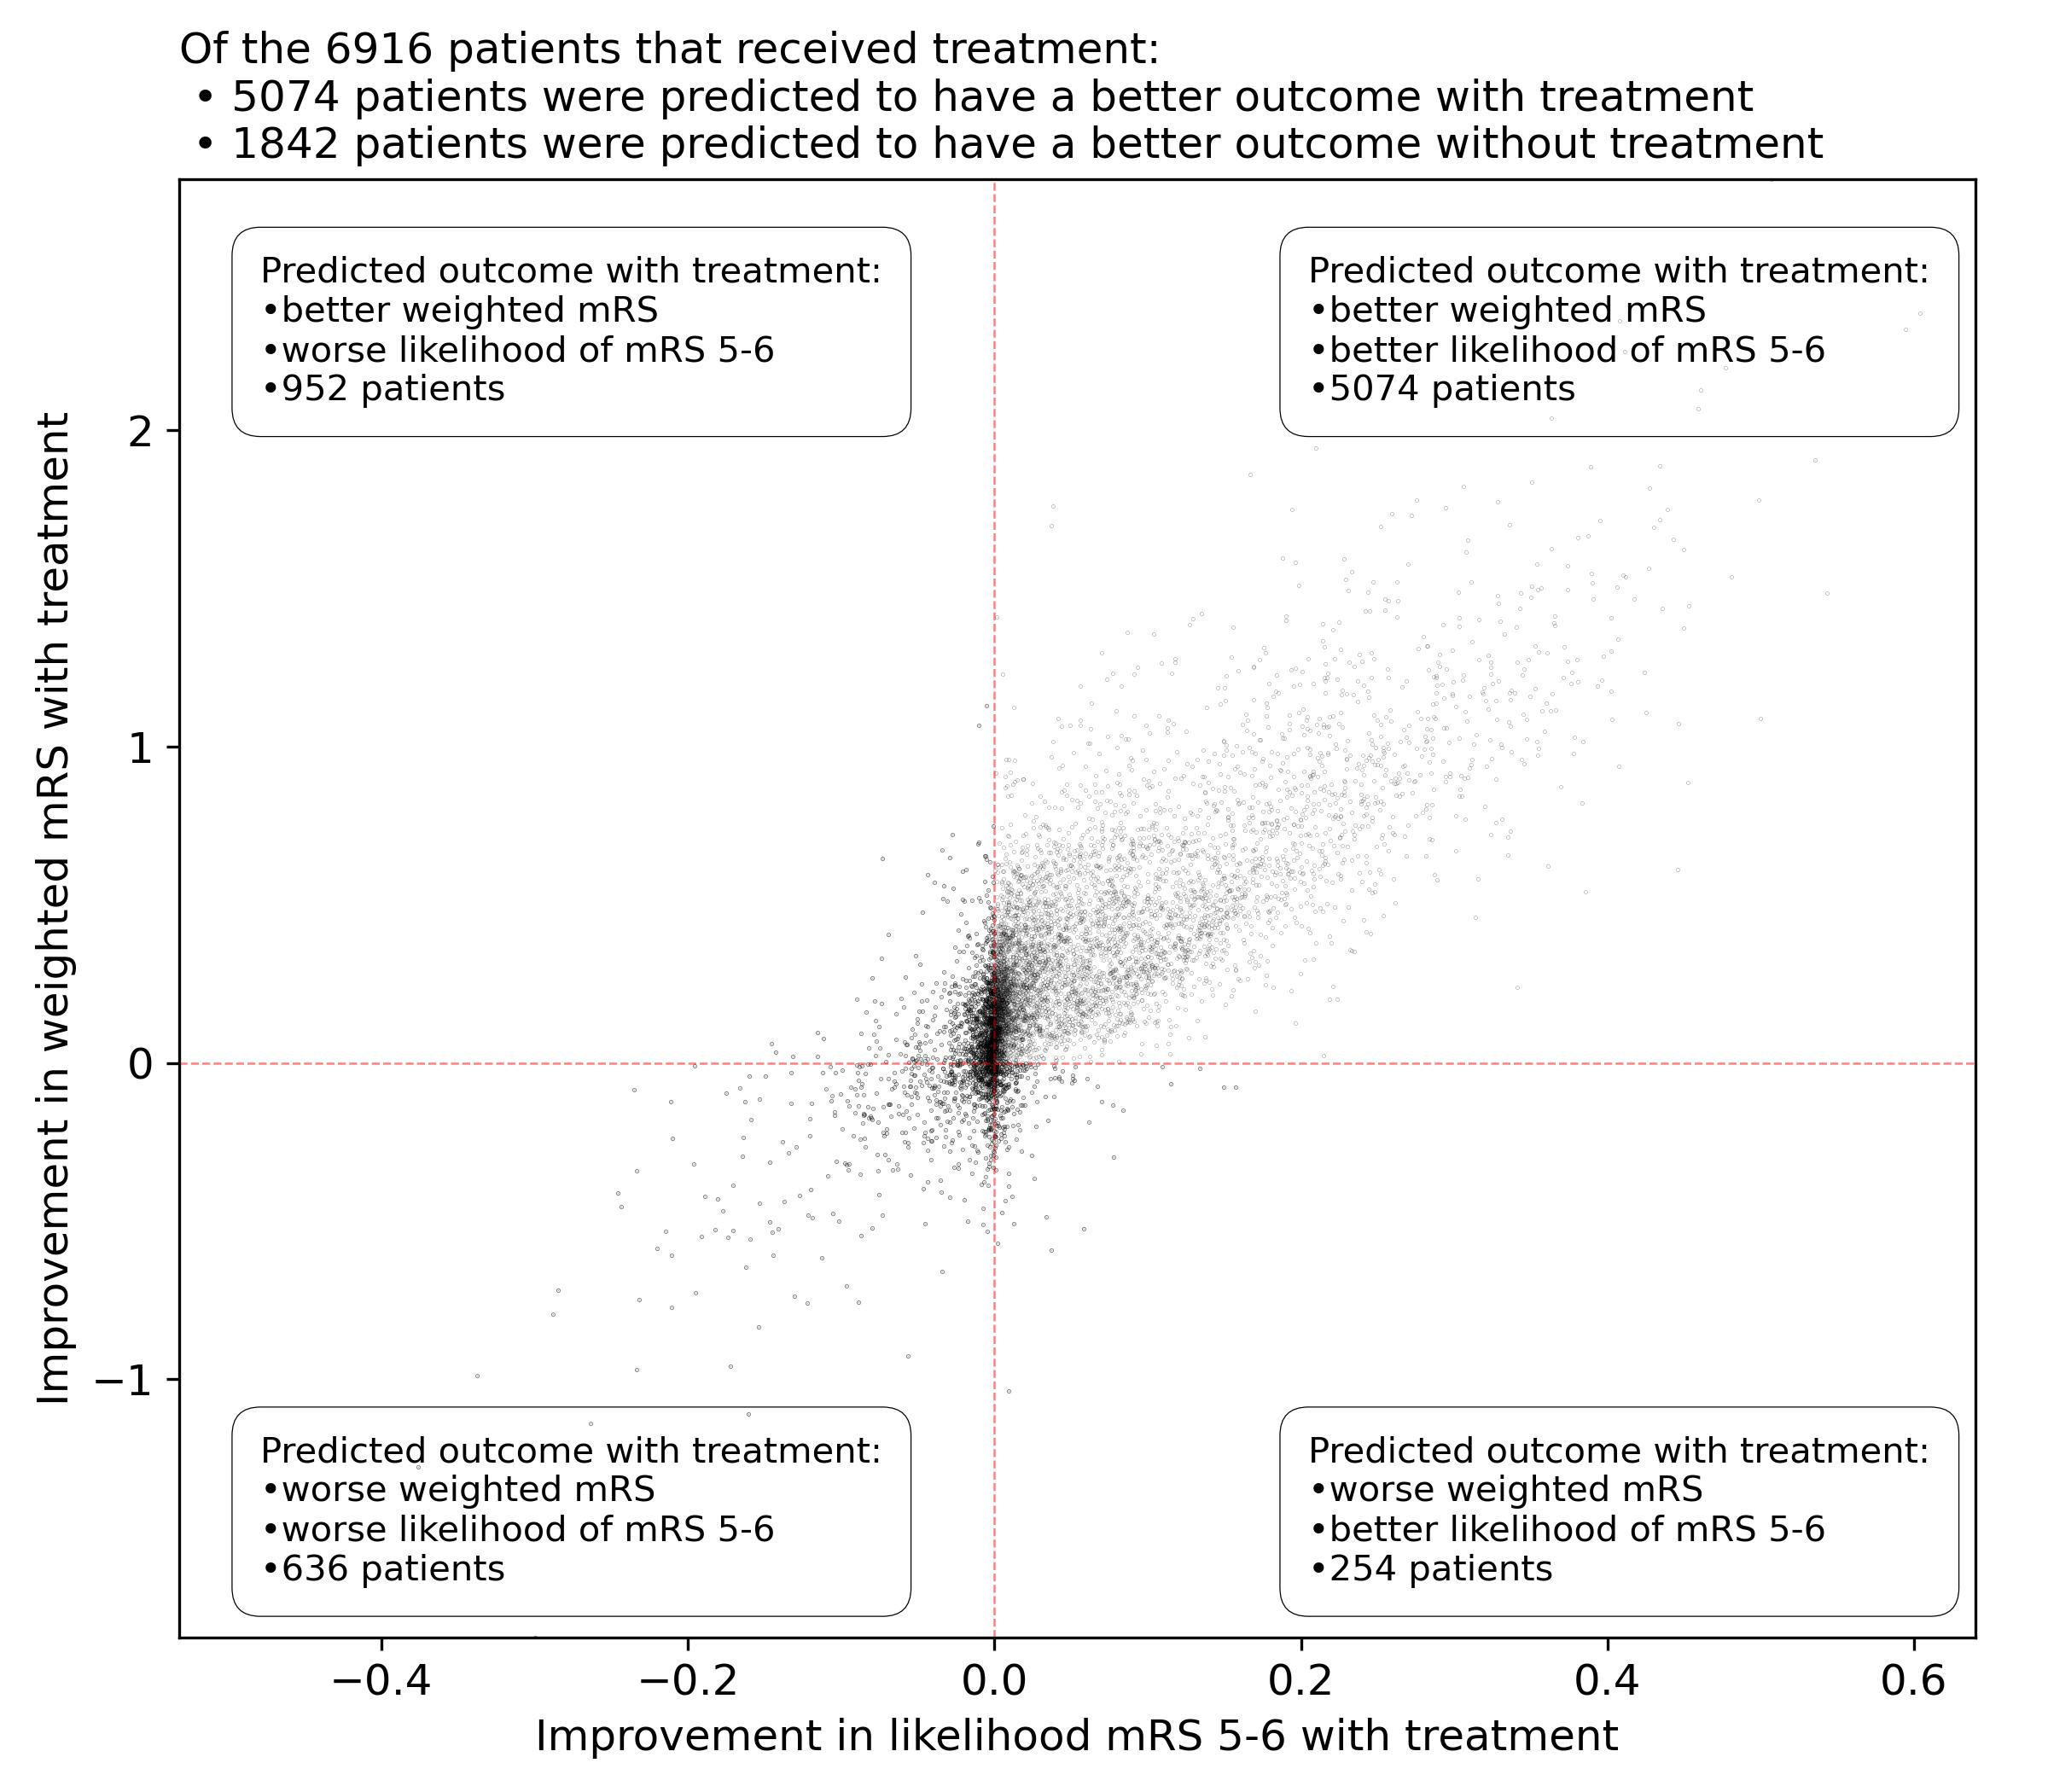
\includegraphics[trim={0 0 0 1.7cm}, clip, width=1\linewidth]{./images/p4_scatter_treated}
      \caption{\footnotesize{Patients who received thrombolysis (n = 6,916)}}
      \label{fig:scatter_receive}
    \end{subfigure}
    
    \vspace{5mm}
    
    \begin{subfigure}{.7\textwidth}
      \centering
      \captionsetup{width=.9\linewidth}
      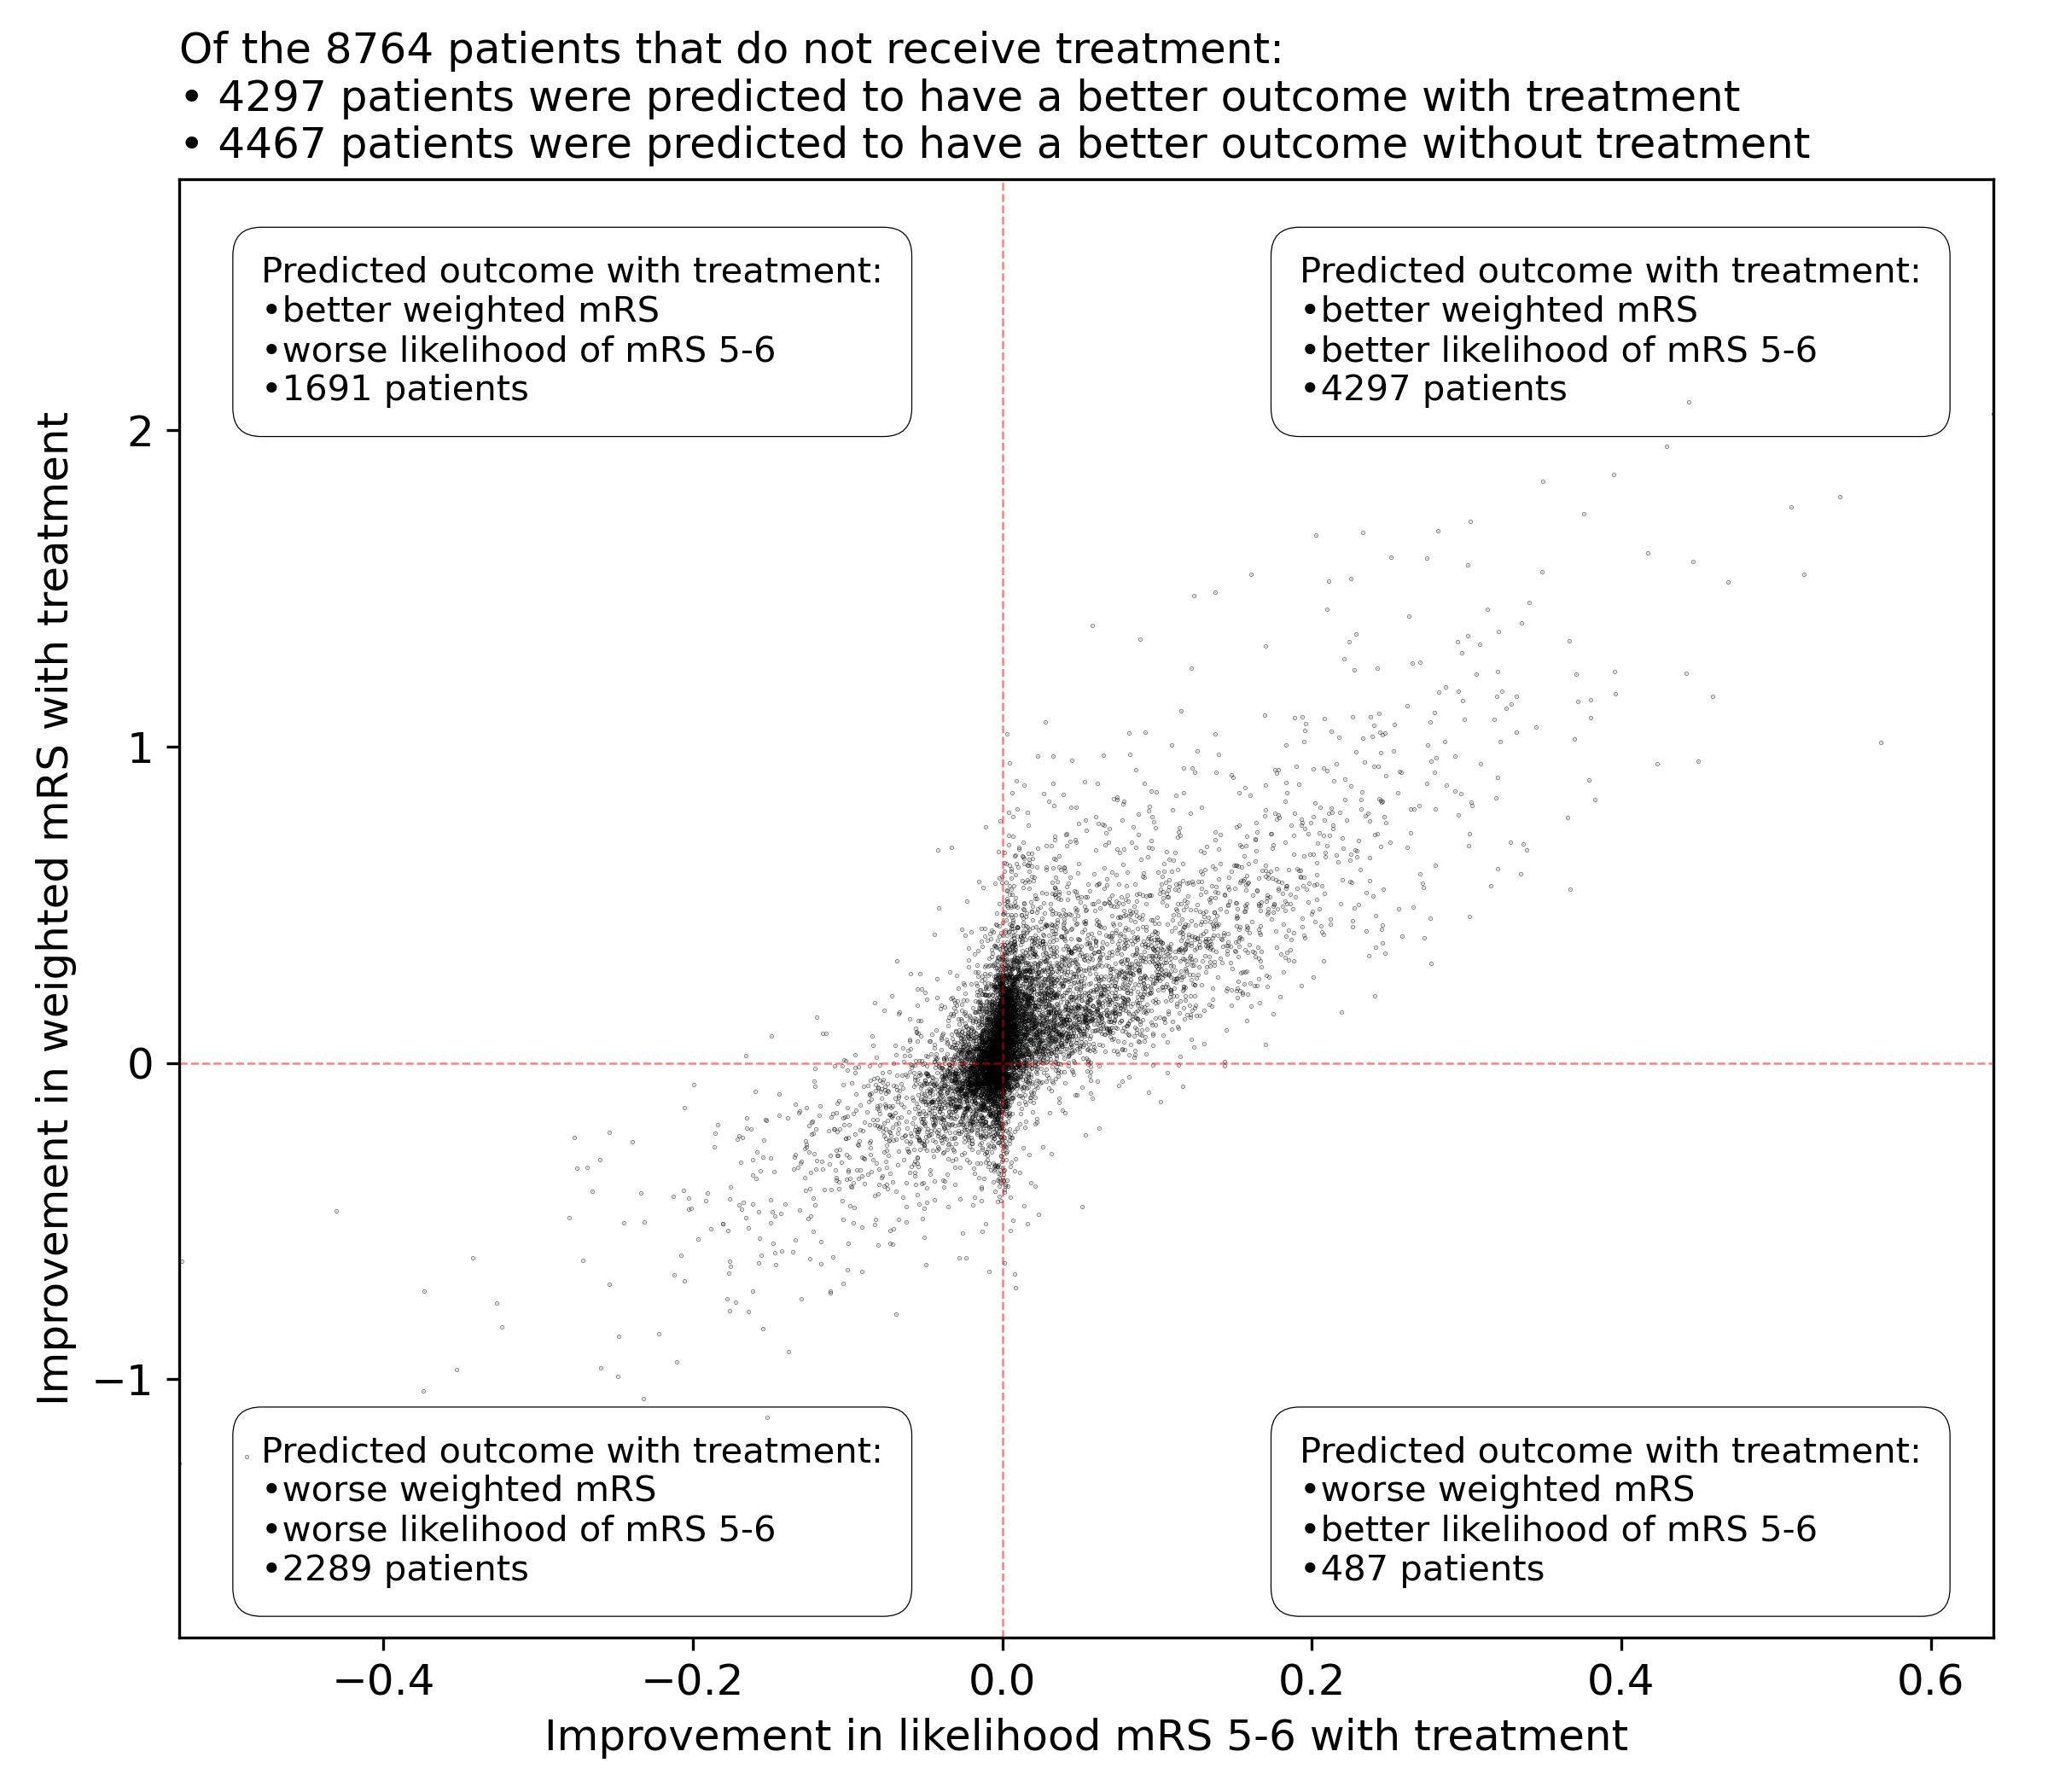
\includegraphics[trim={0 0 0 1.7cm}, clip, width=1\linewidth]{./images/p4_scatter_not_treated}
      \caption{\footnotesize{Patients who did not receive thrombolysis (n = 8,764)}}
      \label{fig:scatter_not_receive}
    \end{subfigure}
  \caption{The predicted benefit or disbenefit of thrombolysis for each of the 15,680 patients in the first k-fold test set. Benefit is shown as both the expected improvement in probability-weighted disability (y-axis) and the improvement in likelihood of avoiding discharge with mRS 5-6. Both measures are expressed so that a positive value is better (a reduction in probability-weighted disability or a reduction in probability of discharge with mRS 5-6). (a) Patients who did actually receive thrombolysis (n = 6,916), (b) Patients who did not actually receive thrombolysis (n = 8,764).}
\label{fig:scatter_all}
\end{figure}
